%Capítulo 3 - Os padrões JPEG e MPEG%

%Forward Error Correction (FEC) = Channel coding%
\thispagestyle{fancy}

``Uma imagem vale mais que mil palavras'', este ditado expressa a importância que os seres humanos dão às informações visuais. Não é de se espantar que existam grandes esforços voltados para pesquisas que objetivam encontrar métodos capazes de avaliar, bem como melhorar a qualidade visual de imagens e vídeos decodificados.

O conhecimento das cacterísticas do sistema visual humano (HVS, do inglês \textit{human visual system}) é fundamental para o desenvolvimento de metodologias eficazes no processo de avaliação e melhoria da qualidade visual de informações visuais. Embora o conhecimento do HVS seja muito limitado, há de se reconhecer que proporcionaram bons resultados, como em \cite{Li_humanvisual} e \cite{5941158}, em que são apresentados dois modelos de quantização adaptativa, um com base na percepção visual humana em determinadas frequências espaciais e temporais e outro que utiliza métricas de qualidade perceptual na fase de estimação de movimentos dos macroblocos, ambos alcançando bons resultados visuais em baixas taxas. Neste contexto, os processos de captura, exibição, armazenamento e transmissão deverão ser adaptados a fim de gerar representações mais exatas das imagens reais.


\section{Artefatos provenientes do processo de compressão}
\label{artefatos}

Na Seção \ref{JPEGeMPEG} foi mencionado que o JPEG e o MPEG-1 realizam uma quantização dos blocos tranformados, a fim de eliminar as redundâncias espacial e temporal. Em alguns sistemas este processo é o principal responsável pelo surgimento de distorções, apesar de não ser o único fator capaz de afetar a qualidade visual. Alguns dos tipos de artefatos mais comuns em sequências de vídeos são listados a seguir:

\begin{itemize}
\item Efeito de blocagem: ocorre devido à quantização independente de blocos, gerando descontinuidade nas fronteiras com blocos adjacentes.
\item Embaçamento: consequência da supressão das componentes de alta frequência durante o processo de quantização, manifestando-se através da perda da resolução espacial.
\item Vazamento de cores: devido aos processos de subamostragem de crominância seguido pela quantização, ocorre o vazamento de cores entre áreas de crominância muito diferentes.
\item Efeito de imagem base da DCT: ocorre quando uma única componente da DCT é dominante em um macro bloco, resultando na ênfase de uma imagem base da DCT.
\item Efeito ressonante: está relacionado com o fenômeno de Gibbs \cite{Gonzalez2006}, logo é mais evidente em áreas de grande contraste. Resultando da irregularidade de reconstrução das componentes de baixa frequência devido ao processo de quantização.
\item \textit{Aliasing}: ocorre quando a frequência de amostragem está abaixo da frequência de Nyquist \cite{Gonzalez2006}, tanto espacial quanto temporalmente.
\end{itemize}

\section{Avaliações subjetiva e objetiva}
\label{ava_subj_obj}

A melhor forma de conseguir avaliar a qualidade de informações visuais é através da opinião de observadores. A nota média de opiniões (\textit{mean opinion score}, MOS), avaliação subjetiva que necessita da opinião de um grupo de observadores, é a melhor forma de avaliar a qualidade de uma imagem se se pretende que essa avaliação seja de acordo com critérios de percepção humana. Porém, este método de avaliação perceptual demanda muito tempo para que se possa coletar um número considerável de opiniões.

Frequentemente o erro médio quadrático (\textit{mean square error}, MSE) é utilizado pelos métodos de avaliação de qualidade de imagens, devido a sua fácil implementação. No entanto, esses métodos apresentam baixo nível de correlação com as avaliações subjetivas, pois o MSE não leva em consideração características espaciais \cite{Wang2006}.

As pesquisas de avaliação objetiva de imagens buscam contornar os inconvenientes presentes na avaliação subjetiva, através de modelos matemáticos que simulam a percepção visual humana.

Há duas abordagens possíveis para o desenvolvimento de simuladores perceptuais: \textit{bottom-up} e \textit{top-down}.

Uma abordagem possível é estudar o funcionamento de cada elemento relevante para a percepção do sistema visual humano de forma a combiná-los em um sistema computacional. Esta abordagem é comumente conhecida como \textit{bottom-up}.

A outra abordagem possível é conhecida como \textit{top-down}, em que  o sistema é tido como uma caixa preta onde comportamentos hipotéticos são implemenados e ajustados. Os pontos atrativos desta abordagem são que o único conhecimento prévio necessário é a relação entre a entrada e a saída do sistema e a simplicidade de implementação.

\section{Classificação das métricas de avaliação de qualidade visual}
\label{metri_obj}

Segundo a disponibilidade de uma imagem de referência, para que uma métrica seja realmente útil para a avaliação de qualidade visual é necessário que ela seja capaz suprir as limitações do MSE. Logo, surgiram vários métodos que, a grosso modo, podem ser classificados em três categorias:

\begin{itemize}
\item Referência completa: há uma imagem de referência (considerada sem distorção) para avaliar uma imagem distorcida. Portanto, proporciona resultados mais precisos em relação a similaridade e fidelidade entre as duas imagens.
\item Sem referência: utilizada quando não é possível ter acesso a imagem referência, logo a avaliação da imagem distorcida deve ser feita as ``cegas'', o que faz disso uma tarefa difícil. Por isso esta categoria também é conhecida como de referência cega.
\item Referência reduzida: neste caso a imagem de referência não está completamente disponível e sim algumas características, que são embutidas no sistema que irá avaliar a imagen distorcida.
\end{itemize}

Outra classificação possível seria em relação à utilização das características do HVS. Neste caso, existem duas categorias:

\begin{itemize}
\item Perceptuais: são formulações matemáticas de certa complexidade inspiradas em
características fisiológicas e psicovisuais da visão que representam de forma automática a percepção humana perante uma representação de uma informação visual, com expressiva correlação com a real percepção humana.
\item Não perceptuais: não utilizam características do HVS nas suas formulações e têm como virtude a baixa
complexidade computacional. Porém, possuem baixa correlação com as avaliações subjetivas.
\end{itemize}

A seguir serão apresentadas métricas não perceptuais e perceptuais de especial interesse para este trabalho.

\subsection{Não perceptuais}
\label{nao_percep}

\subsubsection{Erro médio quadrático (Mean Square Error - MSE)}
\label{mse}

O MSE é uma métrica bastante utilizada que consiste no valor esperado do quadrado do erro,
\begin{equation}
MSE = E \left[ (y(i,j) - x(i,j))^2 \right]
\end{equation}
em que $ y $ é a imagem distorcida, $ x $ é a imagem de referência e $ (i,j) $ determina a posição dos pixels.
\subsubsection{Razão Sinal-Ruído (Signal-to-Noise Ratio - SNR)}
\label{snr}

Quantifica o quanto um sinal foi distorcido através do cálculo da razão entre a energia do sinal e a energia do erro associado à imagem distorcida.


A SNR é comumente medida em dB da seguinte forma,
\begin{equation}
SNR = 10\log_{10}{\frac{\sum_{i,j}[x(i,j)]^2}{\sum_{i,j}[x(i,j)-y(i,j)]^2}}
\end{equation}

\subsubsection{Razão Sinal-Ruído de Pico (Peak Signal-to-Noise Ratio - PSNR)}
\label{psnr}

É normalmente utilizada para medir a qualidade da reconstrução da imagem ou vídeo após uma compressão com perdas.

A PSNR é medida em dB da seguinte forma,
\begin{equation}
PSNR = 10\log_{10}{\frac{NK^2}{\sum_{i,j}[x(i,j)-y(i,j)]^2}}
\end{equation}
onde, $ N $ representa o número total de pixels da imagem e $ K $ representa o valor máximo que um pixel pode atingir. No caso de uma imagem de 8 bits/pixel o valor de $ K $  é 255.

\subsection{Perceptuais}
\label{perceptuais}



\subsubsection{Índice de Similaridade Estrutural (Structural Similarity Index - SSIM)}
\label{ssim}

O SSIM talvez seja a função de aproximação perceptual humana mais utilizada, devido a sua baixa complexidade de implementação em relação às demais e obter boas aproximações do HVS. Esta métrica avalia o quanto a estrutura da imagem de teste é diferente da estrutura da imagem de referência.

O SSIM é definido como
\begin{equation}
SSIM = \left[ l(x,y)^{\alpha}c(x,y)^{\beta}s(x,y)^{\gamma}
\right]
\end{equation}
em que $ \alpha > 0 $, $ \beta > 0 $ e $ \gamma > 0 $ são responsáveis pelo ajuste da importância relativa das
componentes $ l(x,y) $, $ c(x,y) $ e $ s(x,y) $ (correspondentes às componentes de luminância, contraste e estrutura, respectivamente) definidas como
\begin{equation}
l(x,y) = \frac{2 \mu_x \mu_y + c_1}{\mu_x^2 + \mu_y^2 + c_1}
\end{equation}
\begin{equation}
c(x,y) = \frac{2 \sigma_x \sigma_y + c_2}{\sigma_x^2 + \sigma_y^2 + c_2}
\end{equation}
\begin{equation}
s(x,y) = \frac{2 \sigma_{xy}+c_3}{\sigma_x \sigma_y + c_3}
\end{equation}
em que $ \mu_x $ e $ \sigma_x $ são a média e o desvio padrão da imagem $ x $; $ \mu_y $ e $ \sigma_y $ são a média e o desvio padrão da imagem $ y $; $ \sigma_{xy} $ é a covariância entre as imagens $ x $ e $ y $. Os termos $ c_1 $, $ c_2 $ e $ c_3 $ são inseridos com o objetivo de evitar instabilidades.

Esta métrica é aplicada localmente, deslocando, horizontalmente e verticalmente, uma janela de tamanho $B \times B$ sobre a imagem. Pode-se calcular a média do SSIM (MSSIM) para que se tenha uma índice de qualidade geral da imagem, em que $ M $ é o número de janelas e $SSIM_{j}$ é o SSIM associado à j-ésima janela.

\begin{equation}
MSSIM = \frac{1}{M}\sum_{j = 1}^{M}SSIM_{j}
\end{equation}

\section{Quantização inter-adaptativa baseada no HVS}
\label{QIBSVH}

A grosso modo, o sistema visual humano consegue captar pequenas variações de brilho em áreas relativamente grandes, mas não consegue captar com a mesma facilidade quando estas variações estão presentes em componentes de alta frequência \cite{Kelly1979}. Os sistemas de compressão obtêm vantagens desse fato ao quantizar fortemente as componentes de alta frequência e de maneira mas branda as componentes de baixa frequência. Como pode ser visto na figura \ref{fig:dct_comp_distr}, a DCT agrupa as componentes de baixa frequência no canto superior esquerdo e as de alta frequência no inferior direito do macrobloco transformado, possibilitando a produção de tabela de quantização apropriadas para o propósito mencionado.

\begin{figure}[!ht]
\begin{center}
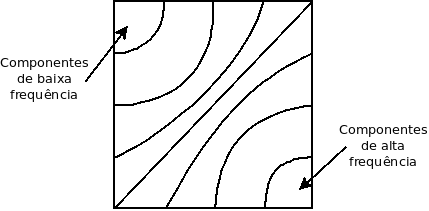
\includegraphics[scale=0.4]{./Figures/png/DCT_COMP.png}
\caption{Distribuição da frequência espacial no domínio da DCT.}
\label{fig:dct_comp_distr}
\end{center}
\end{figure}

O padrão H.261 \cite{telecommunication1993itu} utiliza o mesmo método de compressão para as imagens intra e inter codificadas. Atualmente vários métodos que levam em consideração as características do HVS têm sido propostos para melhorar a qualidade do vídeo reconstruído. 

Em \cite{Li_humanvisual}, um algoritmo de quantização inter adaptativo é proposto. Este algoritmo baseia-se no modelo apresentado por D. H. Kelly \cite{Kelly1979}, o qual afirma que o sistema visual humano é mais sensível às variações de contraste nas frequências espaciais intermediárias, ao passo que é menos sensível em frequências baixas e altas (Fig. \ref{fig:threshold_surface}). 
\begin{figure}[!ht]
\begin{center}
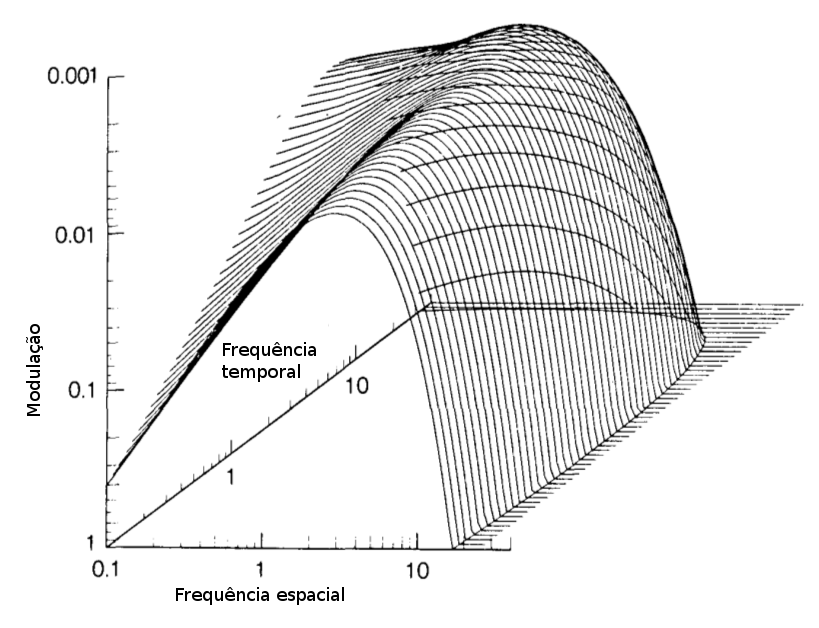
\includegraphics[scale=0.4]{./Figures/png/spatialtemporal_threshold.png}
\caption{Visão perspectiva da superfície de limiar espacial e temporal \cite{Kelly1979}. Cada curva representa a resposta à frequência espacial em uma frequência espacial fixa.}
\label{fig:threshold_surface}
\end{center}
\end{figure}
Tal algoritmo gera matrizes com base nas limitações do HVS em relação às respostas espaciais e temporais ao propor uma equação que representa a resposta do HVS à frequência temporal em função da velocidade e da frequência espacial do macrobloco,
\begin{equation}
G(\alpha,v) = \left[ 6.1 + 7.3 |\log(v/3)|^3 \right] v \alpha^2 \exp \left[ -2 \alpha (v+2)/45.9 \right]
\end{equation}
em que $ v $ velocidade do macrobloco, medida em graus por segundo, e $ \alpha $ é a frequência espacial medida em ciclos por segundo. Ambas são definidas por
\begin{equation}
v = (v_H^2 + v_T^2)^{1/2} 
\end{equation}
\begin{equation}
\quad \alpha_{ij} = \alpha_i + \alpha_j
\end{equation}
em que $ v_H $ e $ v_T $ são as componentes horizontal e vertical da velocidade do macrobloco e $ \alpha_i $ e $ \alpha_j $ são as componentes vertical e horizontal da frequência espacial. Ambas são definidas por
\begin{equation}
v_H = \frac{m_H}{w} \times f \quad \textrm{e} \quad v_T = \frac{m_T}{h} \times f
\end{equation}
\begin{equation}
\alpha_i = \frac{m_H}{m} \times \frac{w}{m} \times c_i \quad \textrm{e} \quad \alpha_j = \frac{m_T}{m} \times \frac{h}{m} \times c_j
\end{equation}
\begin{equation}
c_i = 0.5i \quad \textrm{e} \quad c_j = 0.5j \quad i,j = 1,0...7
\end{equation}
em que $ m_H $ e $ m_T $ são os valores absolutos das componentes do vetor de deslocamento do macrobloco\footnote{Logo, este método de quantização perceptual só é aplicado as imagens preditas (P, B), cuja qualidade depende diretamente do fator de qualidade das imagens I.}, $w$ e $h$ são as dimensões da imagem, e $m$ é o tamanho do macrobloco.

Com base no que foi mencionado, o modelo proposto em \cite{Li_humanvisual} objetiva melhorar a qualidade subjetiva do vídeo decodificado ao quantizar individualmente cada macrobloco respeitando as características do HVS,
\begin{equation}
\label{eq_qhvs}
Q_{HVS}(i,j) = (m_{H} + m_{T})/p \left( 1 - \frac{ G(\alpha_{ij},v) }{G_{max}} \right)
\end{equation}
em que $ Q_{HVS}(i,j) $ é uma componente do modelo de quantização visual, $ p $ é um parâmetro de ajuste e $ G_{max} $ é o valor máximo de $ G(\alpha, v) $.

Por fim, as matrizes de quantização a serem utilizadas são obtidas somando o modelo de quantização baseado no HVS a matriz de quantização plana.

\begin{equation}\label{perceptual_quant}
Q = Q_{flat} + Q_{HVS}
\end{equation}

Portanto, espera-se que a quantização adaptativa com base na sensibilidade do HVS a diferentes frequências espacial e temporal seja capaz de melhorar a qualidade perceptual dos vídeos decodificados, através da utilização da mesma no lugar da tabela de quantização inter imagens (Fig. \ref{fig:tabela_inter}).